\documentclass[10pt,a4paper]{article}
\usepackage[margin=14mm,top=11mm,bottom=11mm]{geometry}
\usepackage[T1]{fontenc}
\usepackage[utf8]{inputenc}
\usepackage{lmodern}
\usepackage{graphicx}
\usepackage{booktabs}
\usepackage{enumitem}
\usepackage{xcolor}
\usepackage{titlesec}
\usepackage{multicol}
\usepackage[hidelinks]{hyperref}
\usepackage{microtype}
\usepackage{caption}
\captionsetup{font=small,labelfont=bf,skip=3pt}
\setlist{nosep,leftmargin=1.2em}
\titlespacing*{\section}{0pt}{6pt}{2pt}
\titlespacing*{\subsection}{0pt}{4pt}{1pt}
\titleformat{\section}{\normalfont\large\bfseries\color{teal!60!black}}{}{0pt}{}
\titleformat{\subsection}{\normalfont\normalsize\bfseries}{}{0pt}{}
\definecolor{crit}{RGB}{0,110,90}
\newcommand{\crit}[1]{\textcolor{crit}{\textbf{[#1]}}}
\pagestyle{empty}

\begin{document}

\begin{center}
{\LARGE\bfseries X3D Copilot}\\[2pt]
{\large A spec-grounded, AI-assisted X3D 4.0 editor that runs entirely in the browser}\\[4pt]
Alberto Jaspe-Villanueva \quad King Abdullah University of Science and Technology (KAUST)\\
\href{mailto:alberto.jaspe@kaust.edu.sa}{alberto.jaspe@kaust.edu.sa}\\[3pt]
\small Live tool: \url{https://albertojaspe.net/x3d-copilot/} \quad
Source (MIT): \url{https://github.com/ajaspe/x3d-copilot} \quad
Video: \textit{see EasyChair form}\\[2pt]
\small\textit{Web3D 2026 -- Web3D/Metaverse Tools Competition. Tool type: editor + validator + converter. Domain: education, content creation, research, standards conformance.}
\end{center}
\vspace{-2pt}

\section{Problem}
Writing X3D by hand is unforgiving: a misspelled field, a \texttt{ROUTE} to a non-existent event, a \texttt{Material} placed directly inside a \texttt{Shape}, or an interpolator with mismatched \texttt{key}/\texttt{keyValue} counts silently produce an empty or wrong scene. Large language models can draft X3D quickly, but left alone they invent fields, mix up X3D versions and never see what they produced. Existing X3D editors are desktop applications with no assistant, and generic AI chat tools have no notion of the ISO/IEC 19775-1 specification. \textbf{X3D Copilot closes this gap}: a zero-install web editor in which every change, whether typed by a human, generated by an AI or dragged with a gizmo, is checked against the official X3D~4.0 schema, a semantic linter derived from the X3D Unified Object Model, and the X\_ITE runtime, and where the AI is forced to work through those same checks until the scene is valid and \emph{looks} right.

\section{What the tool does}
\begin{multicols}{2}
\begin{itemize}
\item \textbf{Live editing} \crit{editor, animation, shaders}: CodeMirror~6 source pane with X3DUOM-driven autocompletion (node names, allowed children per parent, fields with types/defaults/descriptions) next to an X\_ITE~16 view with Phong/Gouraud/flat/wireframe shading, view-all and PNG capture. Animation, sensors, HAnim, PBR (\texttt{PhysicalMaterial}) and \texttt{Script} nodes render live.
\item \textbf{Three validation layers} \crit{X3D adherence, error handling, test cases}: (1)~well-formedness and XSD validation against \texttt{x3d-4.0.xsd} using libxml2 compiled to WebAssembly; (2)~a semantic linter with $\approx$30 rules the schema cannot express (DEF/USE integrity, ROUTE node/field/access/type checks, wrong parent field, SFNode multiplicity, value arity and ranges, interpolator consistency, missing Viewpoint, unknown nodes and fields with did-you-mean suggestions); (3)~X\_ITE runtime errors and warnings captured from the browser. Issues are listed with line numbers and shown inline in the editor; clicking one jumps to the source.
\item \textbf{Direct manipulation} \crit{user-friendly interface}: click any geometry to select its innermost \texttt{Transform}; an X3D-native gizmo (PlaneSensor/CylinderSensor handles injected at runtime, never written to the file) moves, rotates and scales it; an inspector exposes translation, Euler rotation and scale with scrubbing; changes are written back as minimal attribute edits, and the text cursor selects nodes in the view.
\item \textbf{AI co-author} \crit{originality, extensibility}: Google Gemini or Anthropic Claude, called from the browser with the user's key, can only act through tools: read the scene, apply exact text patches, replace the scene, validate, \emph{look up nodes in the ISO spec database}, and take a screenshot. Every edit returns the full validation report, so the model repairs its own mistakes, then inspects the render. The selected node is passed as context (``rotate \emph{this} by 45$^\circ$'').
\item \textbf{Import/export} \crit{converter, configurability}: drag-and-drop glTF/GLB, OBJ, STL, PLY, SVG, VRML and X3D JSON are converted to X3D XML through X\_ITE's loaders and become editable source; export as X3D XML (as edited or canonical), Classic VRML, X3D JSON and PNG.
\item \textbf{Zero infrastructure} \crit{performance, accessibility}: a static site; nothing leaves the browser except the model API calls. Loads in about a second; validation of a typical scene takes tens of milliseconds.
\end{itemize}
\end{multicols}
\vspace{-6pt}

\begin{figure}[h]
\centering
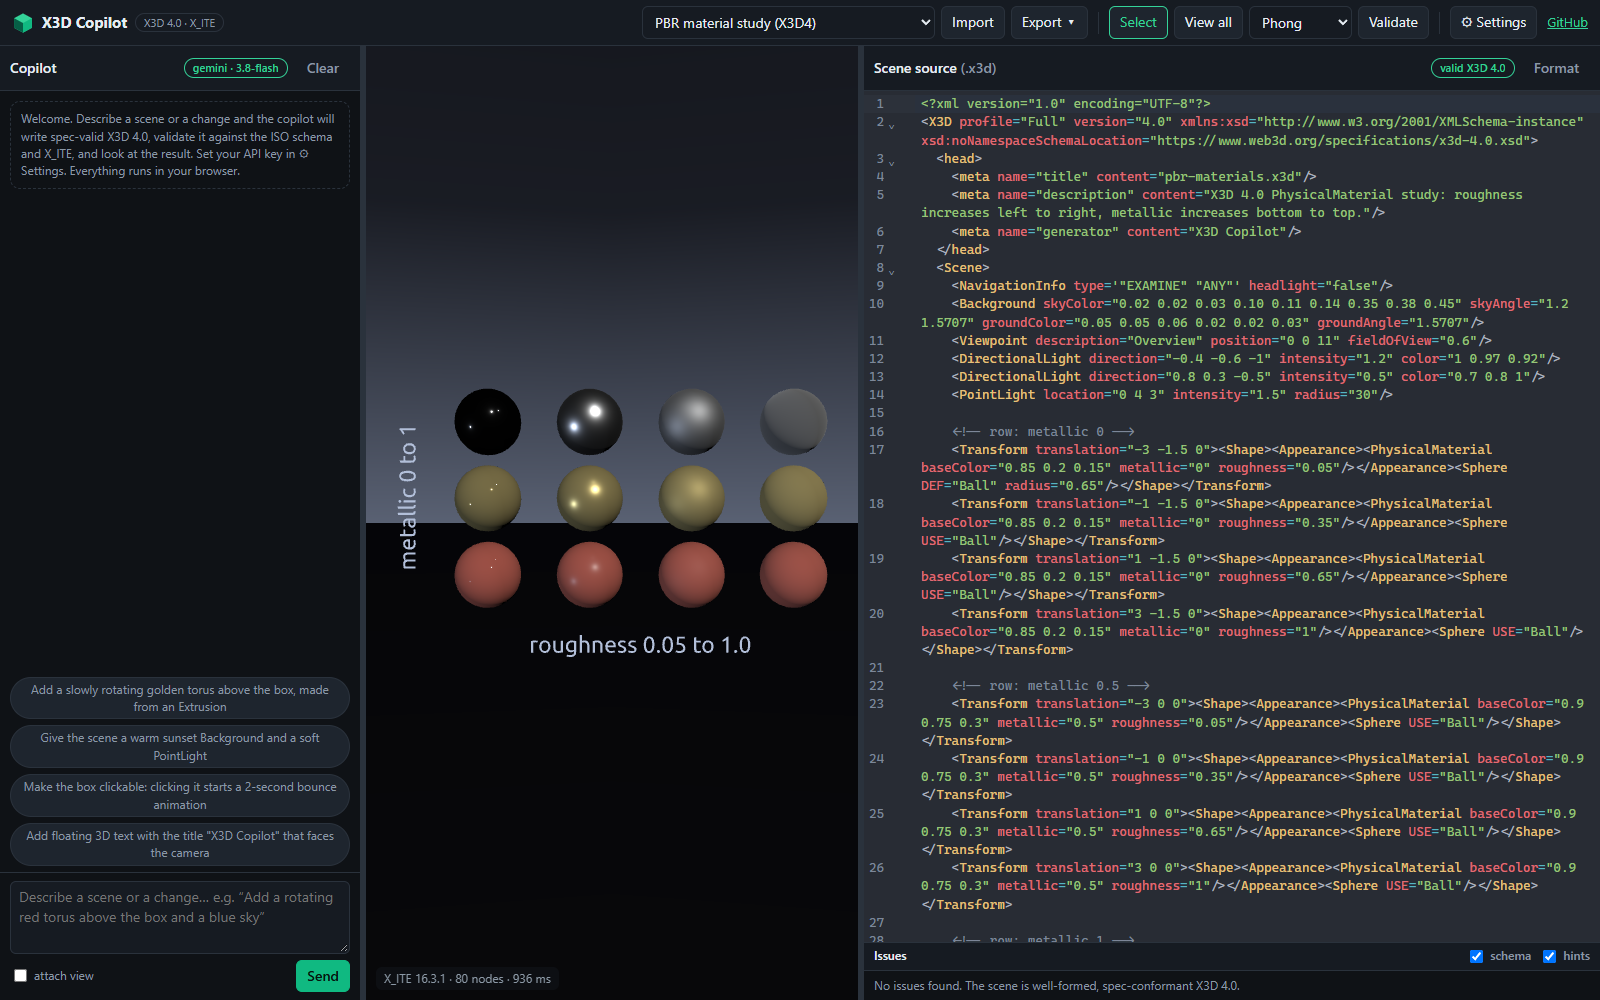
\includegraphics[width=0.46\textwidth]{fig-overview.png}\hfill
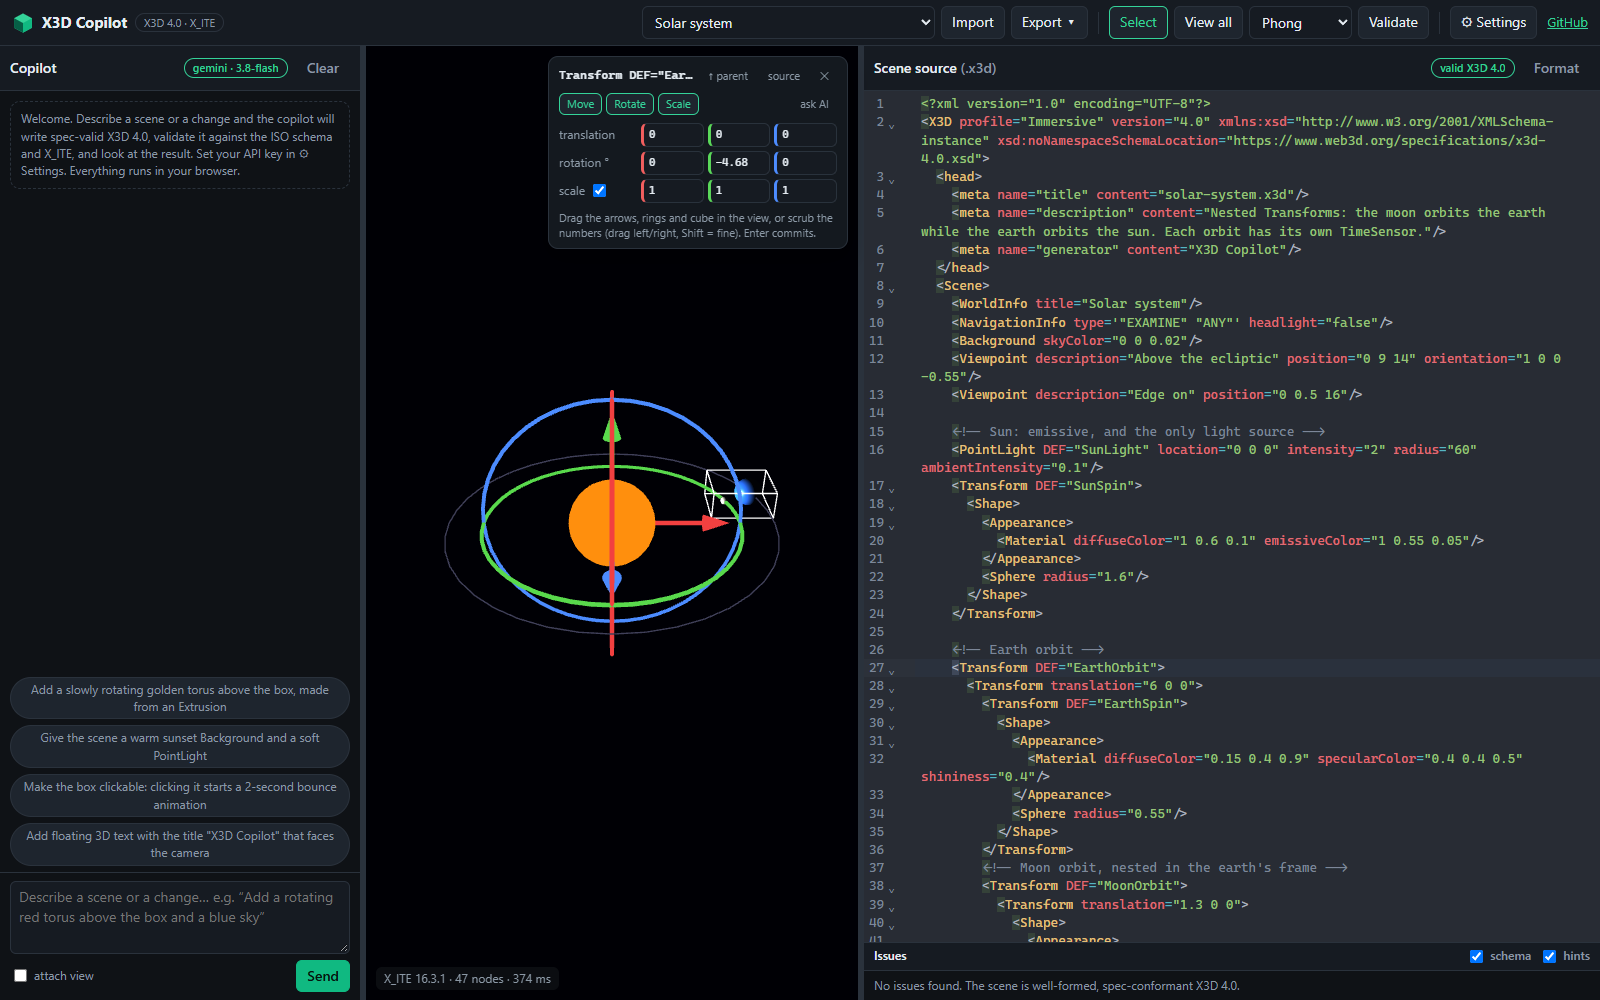
\includegraphics[width=0.46\textwidth]{fig-gizmo.png}
\caption{Left: the three panes -- copilot chat, X\_ITE view, source with inline diagnostics (PBR material study, X3D~4.0 \texttt{PhysicalMaterial}). Right: a selected \texttt{Transform} with the X3D-native gizmo and the inspector; the edited attributes are highlighted in the source.}
\end{figure}
\vspace{-8pt}

\section{X3D standards adherence}
X3D Copilot is built \emph{from} the standard rather than around it. The vendored \texttt{x3d-4.0.xsd} (with the Web3D extension schemas) is the schema validator. The X3D Unified Object Model 4.0 (\texttt{X3dUnifiedObjectModel-4.0.xml}) is compiled at build time into a 260-node database that drives autocompletion, the linter's placement and type rules, and the AI's \texttt{lookup\_node} tool, so the assistant reads field definitions, defaults, \texttt{accessType} and \texttt{containerField} from ISO/IEC~19775-1 instead of guessing. Runtime behaviour comes from X\_ITE, an X3D~4.0 browser, and all conversions are its own encoders (XML, Classic VRML, JSON). The tool produces plain, portable \texttt{.x3d} files with nothing proprietary in them.

\section{Error handling, test cases and extensibility}
Errors are graded (error/warning/hint), attributed to their source (xml/lint/schema/runtime) and phrased as actions (``\texttt{<Material>} goes inside \texttt{<Appearance>}''; ``ROUTE type mismatch: SFRotation~$\rightarrow$~SFVec3f''). Schema messages that duplicate a linter finding are demoted to avoid double counting. The repository ships a vitest suite (53 tests): XSD validation fixtures, one test per linter rule, edit-tool patching, and a check that every example scene is lint-clean and schema-valid, including a deliberately broken scene that must trigger nine specific rules. CI runs typecheck, tests and the build on every push; the app is hosted as a static site on the author's website. The architecture is deliberately modular: the spec database, linter, XSD and runtime layers are independent modules; LLM back-ends are $\approx$150-line adapters behind a provider interface (adding another is a single file); tools exposed to the AI are JSON-schema definitions with executors, so new capabilities (e.g.\ HAnim rigging, glTF export) plug in without touching the agent loop.

\section{Evaluation criteria at a glance}
\vspace{-2pt}
\begin{footnotesize}
\setlength{\tabcolsep}{3pt}\renewcommand{\arraystretch}{0.95}
\begin{tabular}{@{}p{0.25\textwidth}p{0.735\textwidth}@{}}
\toprule
\textbf{Criterion} & \textbf{Where X3D Copilot delivers} \\
\midrule
Originality, technical execution & AI grounded in X3DUOM + closed-loop validation (XSD, linter, runtime, screenshot); gizmo expressed in X3D sensors; XSD validation in WebAssembly \\
Ease of use, user-friendly UI & Three-pane layout, natural-language authoring, click-to-select with inspector, examples gallery, inline diagnostics with jump-to-line \\
Configurability & Provider/model/effort, shading modes, issue filters, gizmo modes, resizable panes, proxy base URL \\
Performance & Static site, lazy schema load, incremental validation ($<$50\,ms typical), X\_ITE rendering; no server round-trips except the model \\
Extensibility & Provider adapters, JSON-schema tools, independent validation modules, spec DB regenerated from the official X3DUOM \\
X3D standards adherence & Official \texttt{x3d-4.0.xsd}, X3DUOM 4.0, X\_ITE X3D~4.0 browser, portable \texttt{.x3d}/\texttt{.x3dv}/\texttt{.x3dj} output \\
Error handling & Graded, sourced, actionable messages; did-you-mean suggestions; runtime warnings captured; AI self-repair loop \\
Advanced features (shaders, animation) & PBR \texttt{PhysicalMaterial}/\texttt{UnlitMaterial}, Script, HAnim, interpolators/sensors examples; shading modes \\
Test cases & 53 vitest tests; every example scene validated; deliberately broken scene as regression fixture; CI on every push \\
Open-source accessibility & MIT, GitHub, static hosting at albertojaspe.net, no accounts required beyond the user's own model key \\
\bottomrule
\end{tabular}
\end{footnotesize}

\section{Why it merits consideration}
\textbf{Tool of the Year}: it is a complete, usable, open-source X3D authoring environment that lowers the entry barrier for students and researchers to zero installs, while raising the conformance bar through the standard's own artefacts. \textbf{Innovation of the Year}: to our knowledge it is the first X3D tool where an AI is grounded in the ISO object model and closed-loop validated by schema, linter, runtime and its own screenshot, and the first web X3D editor whose transform gizmo is itself expressed in X3D sensors.

\begin{figure}[h]
\centering
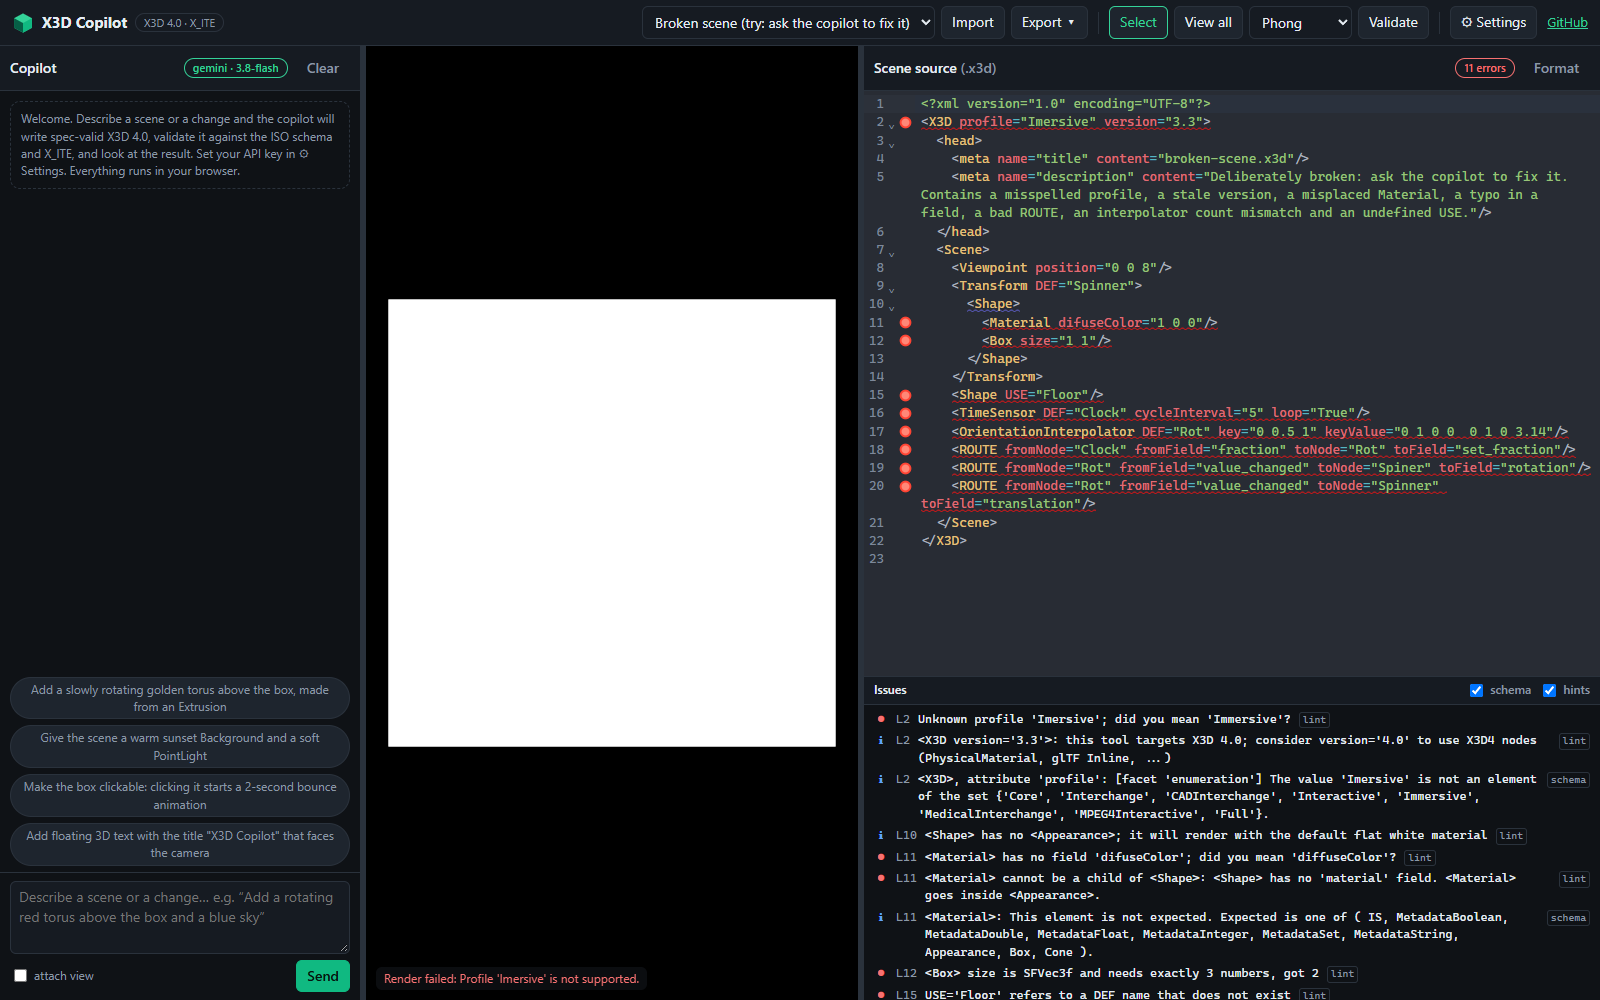
\includegraphics[width=0.44\textwidth]{fig-issues.png}\hfill
\IfFileExists{fig-ai.png}{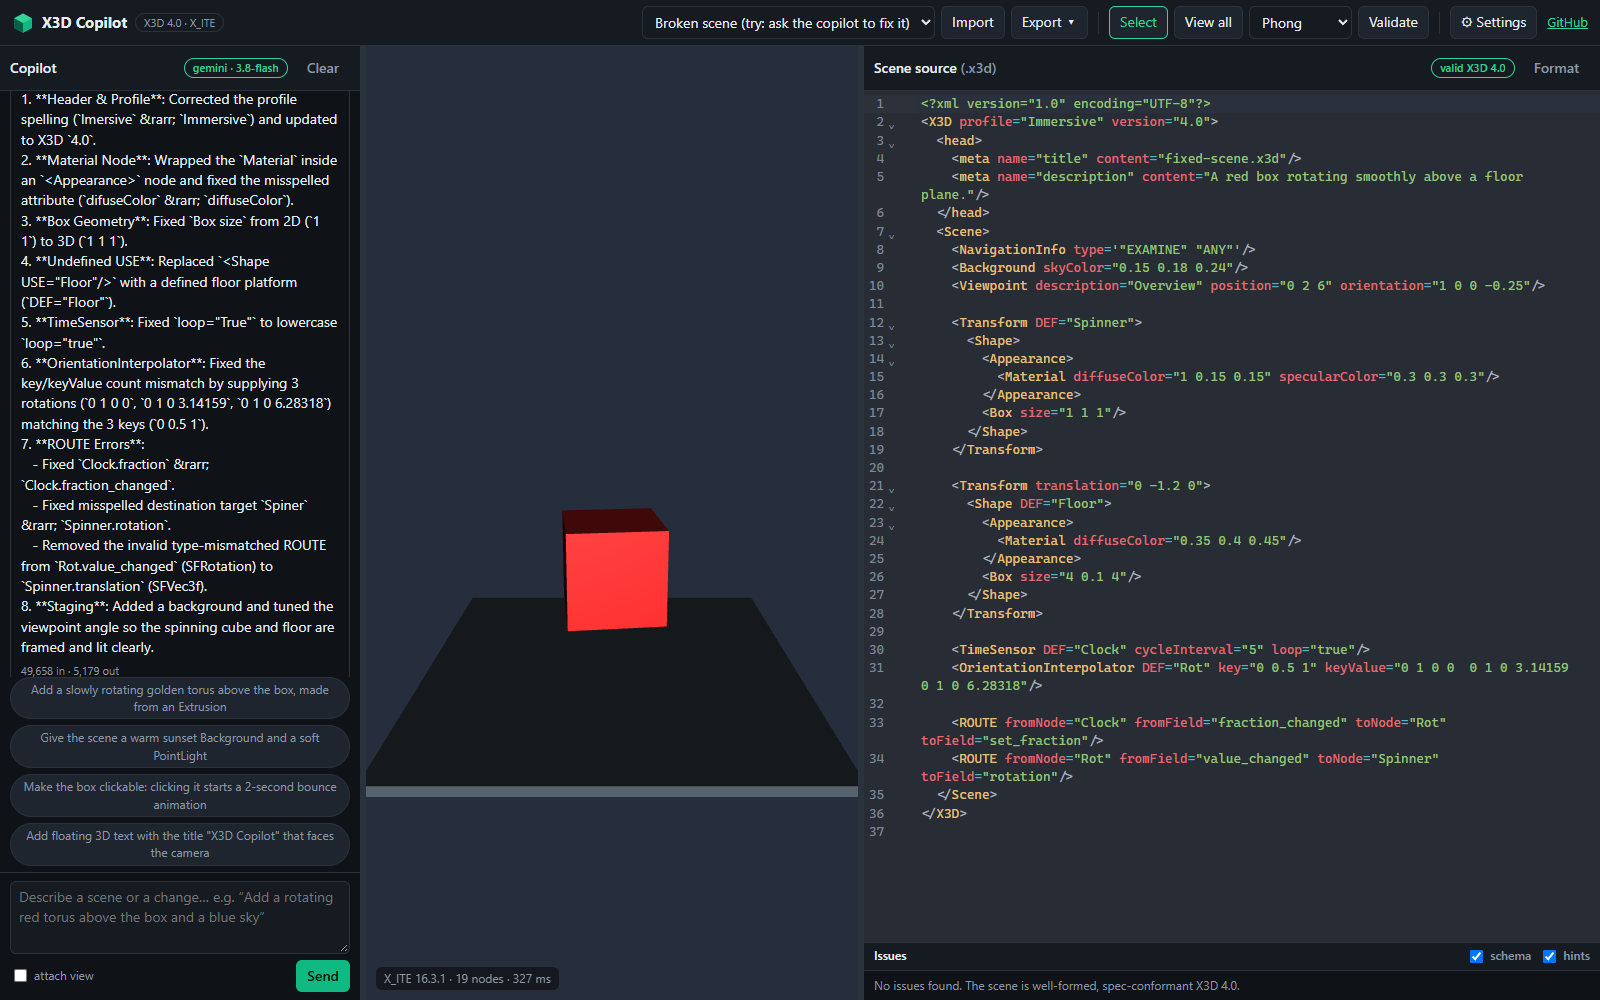
\includegraphics[width=0.44\textwidth]{fig-ai.png}}{\fbox{\parbox[c][0.3\textwidth][c]{0.47\textwidth}{\centering fig-ai.png (run scripts/shots.mjs with GEMINI\_API\_KEY)}}}
\caption{Left: the deliberately broken example -- 11 errors from the three validators with suggestions. Right: the copilot repairing it: read, patch, validate, screenshot, all visible as tool steps.}
\end{figure}

\vspace{-4pt}
\noindent\small Built with X\_ITE (Holger Seelig, MIT), libxml2-wasm, CodeMirror~6, the Google Gen~AI and Anthropic SDKs. Schema and X3DUOM \copyright{} Web3D Consortium. The author thanks the X3D Working Group for maintaining the machine-readable specification artefacts that make this tool possible.
\end{document}
